\chapter{Approches retenues sur la modalité acoustique}
\label{chapitre5}

\section{Motivation}
Dans ce chapitre, nous allons détailler les différentes procédures et tous les questionnements que nous avons eu lors de la réalisation de systèmes de reconnaissance d'émotions dans la parole. Nous utilisons le corpus AlloSat dont nous avons détaillé la création et les caractéristiques dans le chapitre~\ref{chapitre4}.
%Comme nous l'avons vu dans le chapitre~\ref{chapitre3}, le domaine du \textit{Speech Emotion Recognition} continue d'évoluer afin de proposer des systèmes de plus en plus performant.

Dans le cadre de cette thèse, nous nous inscrivons dans un contexte industriel. L'entreprise Allo-Media, partenaire de cette CIFRE, a exprimé des besoins spécifiques quant aux émotions que nous devons traiter. Spécialisée dans le traitement d'informations issues de conversations téléphoniques entre un client et un conseiller, nous sommes inscrit dans ce domaine d'analyse. Comme nous l'avons expliqué dans le chapitre~\ref{chapitre4}, nous avons choisi de nous focaliser sur deux émotions : la satisfaction et la frustration. Ces deux émotions, considérées comme deux émotions opposées dans le cadre de la relation clientèle, sont d'autant plus significatives si l'on analyse leurs évolutions au fil de la conversation. De plus, il nous semblait pertinent de nous concentrer sur l'aspect dimensionnel de l'émotion, afin de mieux alerter et rapporter les points ayant soulevés le plus de satisfaction et de frustration lors de la conversation. Nous rappelons ici que ce type de données en français n'existant pas, nous avons collecté le corpus AlloSat que nous utilisons.

Plusieurs facteurs ont guidés les choix que nous avons mis en place dans nos systèmes de reconnaissance. Tout d'abord, nous faisons face à du signal de basse qualité, puisque provenant d'une source téléphonique. Ensuite nous avions les problématiques de données personnelles dont nous avons parlé au chapitre~\ref{chapitre4}. De plus, nous avons des conversations tenues en français. Et enfin il faut considérer le temps de traitement qui ne doit pas être trop long pour pouvoir être retourné au client rapidement après la fin de la conversation.

La problématique de reconnaissance de ces émotions précises dans un espace continu et ces contraintes nous ont conduit à mener plusieurs expérimentations, tout en considérant les solutions industrielles qui peuvent en découler.

\section{Construction d'une alerte sur les prédictions discrètes}
Le corpus étant annoté de façon discrète et continue, nous nous sommes posé la question de la pertinence de ces deux annotations dans le cadre industriel. En effet, un système de reconnaissance portant sur les étiquettes discrètes est plus facile à mettre en place et moins coûteux en ressources, puisque nous avons moins d'étiquettes à prédire. Dans le cas de l'émotion continue, on ne prédit pas d'étiquette, il est donc difficile de comparer les deux approches. Cependant quelque soit la durée de la conversation, seules trois étiquettes sont à prédire : le niveau de frustration/satisfaction de début, de fin de conversation et son type d'évolution entre les deux.

Nous avons donc considéré dans un premier temps une prédiction d'étiquettes discrètes. En effet, cela nous permettait d'avoir une première approche sur la satisfaction et la frustration qui peut être utilisée dans un contexte industriel. Nous avons imaginé un système d'alerte permettant de mettre en avant les conversations dites \emph{préoccupantes}, que nous avons détailler dans la prochaine section. On appelle préoccupantes, les conversations ayant une résolution (soit une fin) annotée en frustration.

%Notre premier travail préliminaire, afin de juger de la difficulté de la tâche et de la pertinence du corpus, a été de mettre en place une alerte sur les conversations dites \emph{préoccupantes}.
Nous avons donc mis en place une classification supervisée de reconnaissance de la satisfaction et de la frustration discrète. Nous avons tout d'abord cherché à prédire l'étiquette de fin de conversation. Comme les étiquettes de début de conversation ne contiennent quasiment que des états neutres, il ne nous semblait pas constructif de construire un système de classification autour de ces données.

\subsection{Les descripteurs}
Pour mettre en place cette alerte, nous avons fait le choix de travailler avec plusieurs ensembles de descripteurs. En effet les états émotionnels sont détectables à la fois dans l'acoustique et la linguistique. Ces descripteurs sont décrits dans le tableau~\ref{tab:descripteursDiscrets}.

\begin{table}[h]
  \centering
\begin{tabular}{|l|l|l|l|l|}
\hline
Nom         & Modalité                                                             & Contient                                                   & \begin{tabular}[c]{@{}l@{}}Nombre features \\ avant réduction\end{tabular} & \begin{tabular}[c]{@{}l@{}}Nombre features\\ après réduction\end{tabular} \\ \hline
Audio       & acoustique                                                           & IS2009~\cite{OPENSMILE}                       & 384                                                                        & 100                                                                       \\ \hline
Texte       & linguistique                                                         & TF-IDF                                                     & 4000                                                                       & 100                                                                       \\ \hline
Audio+Texte & \begin{tabular}[c]{@{}l@{}}acoustique\\ et linguistique\end{tabular} & \begin{tabular}[c]{@{}l@{}}IS2009 et\\ TF-IDF\end{tabular} & 200                                                                        & 200                                                                       \\ \hline
\end{tabular}
\caption{Description des trois ensembles de descripteurs utilisés pour réaliser la reconnaissance des émotions discrètes des fin de conversations.}
\label{tab:descripteursDiscrets}
\end{table}


La modalité acoustique est représentée par l'ensemble de référence IS2009 contenant 384 descripteurs, décrit dans le chapitre~\ref{chapitre3}~\cite{OPENSMILE} et la modalité linguistique par un TF-IDF contenant 4000 descripteursn aussi décrit au chapitre~\ref{chapitre3}. Comme le nombre de descripteurs est très grand pour une classification de 303 documents, nous avons décidé de faire de la sélection de descripteurs afin d'éviter le sur-apprentissage notamment~\cite{Tahon2016}. Cette sélection de type ranking est effectuée avec l'outil scikit-learn~\cite{scikitlearn} selon un seuil de variance (feature\_selection.VarianceThreshold) et un classement de \textit{mutual information} (feature\_selection.RFE).

Nous avons également fait le choix de considérer les deux modalités en même temps, en fusionnant les deux ensembles de descripteurs. Pour la fusion, nous avons concaténé les deux vecteurs de descripteurs. Pour cette fusion nous avons testés différentes modalités de normalisation et nous avons choisi de conserver la normalisation standard (à chaque valeur on soustrait la moyenne et on divise par l'écart type) puisqu'elle donne les meilleurs résultats.

\subsection{Modèles et protocole d'apprentissage}
En ce qui concerne les systèmes de Machine Learning mis en place, nous avons décidé d'utiliser la régression logistique et un SVM que nous avons décrit au chapitre~\ref{chapitre2}. Ces choix proviennent de précédentes expérimentations que nous avions mis en place sur une classification antérieure qui ne sera pas présentée dans ce manuscrit. Suite à une non-conformité avec le réglement général de protection des données, nous avons du supprimer des données et les expérimentations qui avaient été menées avec. Ces deux classifieurs sont implémentés en utilisant l'outil scikit-learn également. %Pour plus d'information sur leur configuration, le code de cette classification est disponible en annexe~\ref{an:codeFirstClassif}.

La classification se fait en validation croisée (\textit{k-folds}) avec $k=5$, c'est à dire que nous avons divisé les conversations du train et du dev en $k$ échantillons. Pour chaque pli, l'ensemble de validation va changer, une fois l'apprentissage terminé. On va donc faire cinq apprentissages. Le score final correspond à la moyenne des scores de ces cinq scores de performance. Ce procédé est très utilisé pour éviter le sur-apprentissage, dans le cas où peu de données sont disponibles.

Les modèles ont été évalués avec les mesures de précision et rappel non pondérées, que nous avons introduit au chapitre~\ref{chapitre3}.

\subsection{Résultats et analyse}

\begin{table}[h]
  \centering
  \begin{tabular}{|l| l l l | l l l|}
    \hline
    modèle    &\multicolumn{3}{c|}{Regression Logistique} &\multicolumn{3}{c|}{SVM} \\
    \hline
    modalités    &acoustique  &linguistique  &les deux  &acoustique  &linguistique  &les deux\\
    nb descripteurs         & 100&100&200 & 100&100 &200\\
    \hline
    &\multicolumn{6}{c|}{\textbf{Calcul avec les sept conversations satisfaites}}\\
    \hline
    UAP           &0.31  &\textbf{0.52}  & 0.42 &0.36 &0.44  &0.40 \\
    UAR              &0.35  &\textbf{0.52}  &0.46 &0.39  &0.48  & 0.45\\
    %fscore              &0.324  &0.505  &0.432  &0.365 &0.459  &0.422 \\
    \hline
    %                   &&audio    &&text     &&both \\
    %per classes on LR  &sat &neu &fru &sat &neu &fru &sat &neu &fru \\
    %precision           &infini(0/0) &0.54 &0.38 &inf &0.7 &0.86 &inf &0.64 &0.61 \\
    %recall              &0 &0.64 &0.4            &0 &0.97 &0.6   &0 &0.82 &0.55 \\
    %per classes on SVM  &sat &neu &fru &sat &neu &fru &sat &neu &fru \\
    %precision           &infini(0/0) &0.59 &0.5 &inf &0.67 &0.67 &inf &0.63 &0.58 \\
    %recall              &0 &0.82 &0.35            &0 &0.85 &0.6   &0 &0.79 &0.55 \\
    %per classes (LR)  &neu &fru  &neu &fru  &neu &fru \\
    %precision            &0.54 &0.38  &0.7 &0.86  &0.64 &0.61 \\
    %recall              &0.64 &0.4   &0.97 &0.6  &0.82 &0.55 \\
    %per classes (SVM)   &neu &fru  &neu &fru &neu &fru \\
    %precision           &0.59 &0.5  &0.67 &0.67  &0.63 &0.58 \\
    %recall               &0.82 &0.35 &0.85 &0.6  &0.79 &0.55 \\
    &\multicolumn{6}{c|}{\textbf{Calcul sans les conversations satisfaites}}\\
    \hline
    UAP           &0.46 &\textbf{0.78} &0.63 &0.54 &0.67 &0.61 \\
    UAR              &0.52 &\textbf{0.78} &0.68 &0.58 &0.72 &0.67 \\
    \hline
  \end{tabular}
\caption{Scores des systèmes de classification sur l'émotion de fin de conversations. UAP correspond à \textit{unweighted average precision} et UAR à \textit{unweighted average recall}.}
\label{tab:resultClassifDiscrete}
\end{table}


Les  performances des différents modèles sont indiquées dans le tableau~\ref{tab:resultClassifDiscrete}. Nous pouvons observer que la régression logistique donne des meilleurs résultats sur la modalité linguistique et la fusion des deux modalités. Nous voyons également que la modalité linguistique donne toujours de meilleurs résultats. Comme il n'y a que sept conversations satisfaites dans nos jeux de données, nous avons fait le choix de supprimer entièrement la classe satisfaite et de ré-apprendre un système avec deux classes : neutre et frustré. Ce modèle est donc appris avec sept documents de moins que le précédent. Nous observons que par ce procédé, nous améliorons fortement le score, passant d'un maximum de $0.52$ à $0.78$.

Bien que simple, cette première classification nous a permis de confirmer l'importance de la modalité linguistique, dont nous parlerons dans le chapitre~\ref{chapitre6}. Fort de ces expérimentations, nous avons mis en place une reconnaissance des émotions continues.

\section{Reconnaissance continue de la dimension de satisfaction/frustration}
Pour mettre en place cette reconnaissance de l'émotion continue, nous avons choisi dans un premier temps de nous comparer et donc de reproduire les expérimentations des articles de référence~\cite{Schmitt2019,SEWA} et des campagnes AVEC~\cite{AVEC2017,AVEC2018,AVEC2019}. La majorité de ces travaux se portent sur des séquences d'audio de taille fixe. La sous partie de SEWA à laquelle nous avons accès ne comporte que des conversations de durée inférieure à trois minutes. De plus, un padding circulaire est utilisé pour ramener toutes ces conversations à une durée de trois minutes dans la plupart des travaux. Ce positionnement, souvent adopté, permet notamment d'utiliser toutes les architectures neuronales (notamment les CNN). Il est adapté lors que nous avons des données assez homogènes, dans notre cas en terme de durée, comme c'est le cas avec le corpus SEWA.

Comme nous l'avons vu dans le chapitre~\ref{chapitre4}, dans AlloSat les conversations ont des durées variant de 32 secondes à 41 minutes avec une moyenne ($MOY$) de 7m24s et un écart type ($STD$) de 4m58s. Une bonne pratique courante du domaine est de fixer la taille d'entrée à $MOY + STD$ (ici 12m22s) pour couvrir statistiquement plus de 95\% du corpus. Les séquences longues sont alors coupées à $MOY + STD$ tandis que les séquences courtes sont rallongées avec un padding. Dans notre cas, cela reviendrait à traiter des conversations de 12m22s.

Afin de réduire l'effet du padding et la durée d'apprentissage, nous avons décidé de fixer la durée de la séquence d'entrée à sept minutes. Nous avons appliqué un padding circulaire sur les courtes séquences.

En résumé nous avons trois cas possibles :
\begin{itemize}
  \item pour une conversation de durée inférieure à sept minutes : on prend la conversation et on fait un padding circulaire, c'est à dire qu'à la fin de la séquence, on concatène le début de la conversation. Par exemple, pour un document de cinq minutes, nous concaténons les deux premières minutes du document à la suite de la fin de ce dernier,
  \item pour une conversation de durée égale à sept minutes : on prend la conversation en entier, sans traitement,
  \item pour une conversation de durée supérieure à sept minutes : on supprime tout ce qui est au delà des sept minutes.
\end{itemize}

Une fois ce pré-traitement des données mis en place, nous avons commencé par travailler sur les descripteurs accoustiques.

\subsection{Exploration des ensembles de descripteurs GeMAPS}
Pour mieux comparer notre travail avec l'état de l'art dans le domaine du SER, nous avons décidé d'utiliser l'ensemble eGeMAPS~\cite{Eyben2016}, que nous avons détaillé dans le chapitre~\ref{chapitre3}. Pour rappel, cet ensemble est constitué de descripteurs de bas niveau et de fonctions statistiques appliquées sur ces derniers. Cet ensemble regroupe 88 descripteurs.

Dans les travaux de Schmitt et al.~\cite{Schmitt2019}, un sous ensemble, appelé f\_eGeMAPS, a été défini à partir de 23 LLD et des fonctions mathématiques appliquées sur ces LLD (principalement moyenne et STD). Il totalise 46 descripteurs. Un dernier descripteur, fonctionnant comme une détection de voix (\textit{voice activity detection} i.e. vad), dénotant l'identité du locuteur (zéro ou un), est également incluse dans f\_eGeMAPS, portant le nombre de descripteurs à 47. Ce descripteur est directement lié aux choix de concept du corpus SEWA. En effet, il est composé de conversations entre deux personnes qui sont enregistrés dans le même canal, ce qui signifie que pour analyser séparemment les deux interlocuteurs, les conversations sont présentées dans deux documents distincts. Pour dissocier ces deux documents, on utilise le descripteur de vad.

Dans notre travail, les deux ensembles ont été extraits de nos données toutes les 250~ms de manière synchronisée avec le pas d'annotation d'AlloSat avec l'outil OpenEAR~\cite{OpenEAR}, qui s'appuie sur OpenSMILE~\cite{OPENSMILE}. Puisque nous ne gardons que le signal de l'appelant, nous ajoutons un descripteur, appelé \textit{vad}, pour indiquer si l'appelant parle (1) ou non (0). Ce descripteur est déduit des transcriptions automatiques.

Nous avons donc comparé un total de quatre ensembles de descripteurs :
\begin{itemize}
    \item \textbf{eGeMAPS-88} : L'ensemble de descripteurs eGeMAPS, extrait avec OpenEAR par pas de 250~ms,
    \item \textbf{eGeMAPS-89} : Même ensemble que précédemment mais avec l'ajout du descripteur \textit{vad} qui modélise la présence ou l'absence de parole de la part du locuteur.
    \item \textbf{eGeMAPS-46} : Le sous-ensemble de descripteur utilisé par Schmitt et al.~\cite{Schmitt2019}, extrait avec OpenSMILE par pas de 250~ms.
    \item \textbf{eGeMAPS-47} : Même ensemble que précédemment mais avec l'ajout du descripteur \textit{vad} qui modélise la présence ou l'absence de parole de la part du locuteur.
\end{itemize}

Pour réaliser cette reconnaissance, nous utilisons deux réseaux de neurones décrit dans la figure~\ref{fig:biLSTM}. Afin de pouvoir comparer nos résultats avec l'état de l'art, nous avons fait le choix de reproduire le système proposé dans le challenge AVEC 2018~\cite{AVEC2018} sur la modalité \textit{Cross-cultural Affect}. Ce réseau neuronal, correspondant à la figure~\ref{fig:biLSTM} gauche, est composé de deux couches biLSTM de respectivement 64 et 32 neurones. L'architecture bidirectionnelle est utilisée afin notamment d'éviter les problèmes de délai d'annotation. En effet, il est possible que l'annotation présente des délais, le temps que l'annotateur appuie sur les flèches du clavier ou qu'il décide s'il y a vraiment une variation à annoter. Nous avons fixé le nombre d'époque maximum à 200. Le nombre d'époque doit être déterminé par l'expérimentation en elle-même, nous avons donc vérifié à posteriori qu'il n'y avait plus d'amélioration du score après 200 époques. Nous avons controlés jusqu'à 500 époques.

Le second réseau, correspondant à la figure~\ref{fig:biLSTM} droite, est composé de quatre couches biLSTM comme décrit dans~\cite{Schmitt2019}. Les couches de biLSTM sont composées respectivement de 200, 64, 32, 32 neurones. Ce réseau est plus profond, nous avons donc augmenté le nombre d'époque à 500.

Pour ces deux réseaux, la fonction d'activation utilisée est la fonction tangente hyperbolique. Un seul neurone de sortie est utilisé pour prédire une valeur toutes les 250~ms. Comme il s'agit d'une régression et pour être comparable aux articles de référence, on utilise le coefficient de corrélation de concordance (CCC)~\cite{CCC} comme fonction de coût pour l'apprentissage du réseau et comme métrique d'évaluation pour déterminer le meilleur système.
Pour rappel, ce score CCC varie de 0 (probabilité d'un tirage aléatoire) à 1 (corrélation parfaite).

\begin{figure}[thb]
  \centering
  \begin{minipage}[b]{0.49\linewidth}
      \center
      \centerline{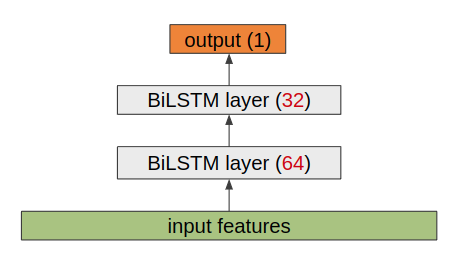
\includegraphics[width=8cm]{./Chapitre5/figures/biLSTM2.png}}
  \end{minipage}
  \begin{minipage}[b]{0.49\linewidth}
      \center
      \centerline{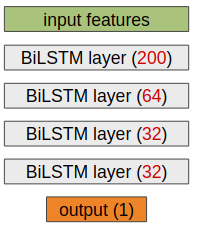
\includegraphics[width=8cm]{./Chapitre5/figures/biLSTM4.png}}
  \end{minipage}
    \caption{Schéma de la configuration des systèmes neuronaux appelés biLSTM-2 (à gauche) et biLSTM-4 (à droite). Le nombre de neurone est indiqué en rouge et entre paraenthèses sur chaque couche. Comme il s'agit de réseaux bidirectionnels, il faut multiplier par deux le nombre de neurones pour avoir le nombre de paramètres réels.}
    \label{fig:biLSTM}
\end{figure}


Ces premiers réseaux sont implémentés avec le framework Keras~\footnote{https://keras.io} en utilisant Tensorflow~\footnote{https://www.tensorflow.org/}. L'apprentissage se fait par batch de neuf conversations en utilisant l'optimiseur ADAgrad~\cite{Duchi2011} dont nous avons parlé au chapitre~\ref{chapitre2}. Les conversations sont mélangées aléatoirement entre chaque époque. Le learning rate est initialisé à 0,001.

Nous avons conservé les poids des réseaux donnant le meilleur score sur le développement afin de prédire les résultats sur le test.


\begin{table}[th]
  \centering
  \begin{tabular}{| l | ll | ll |}
      \hline
      Ensemble de descripteurs & \multicolumn{2}{c |}{\textbf{biLSTM-2}} &\multicolumn{2}{c |}{\textbf{biLSTM-4}} \\
      & dev & test & dev & test \\
      \hline
      eGeMAPS-88 &0.510 &0.363 &\textbf{0.666} &0.431 \\
      eGeMAPS-89 &\textbf{0.549} &\textbf{0.365} &0.619 &\textbf{0.542} \\
      f\_eGeMAPS-46 &0.469 &0.260 &0.607 &0.354 \\
      f\_eGeMAPS-47 &0.508 &0.359 &0.574 &0.422 \\
      \hline
  \end{tabular}
  \caption{Score CCC des systèmes de reconnaissance des émotions en utilisant quatre ensembles de descripteurs différents et deux architectures neuronales sur les ensembles de développement et de test d'AlloSat.}
  \label{tab:result7minutes}
\end{table}


Le tableau~\ref{tab:result7minutes} donne un résumé des résultats obtenus avec les modèles et les ensembles de descripteurs étudiés.
Nous pouvons remarquer que l'ensemble eGeMAPS-88 et 89 nous donne de meilleurs résultats sur les deux architectures neuronales que f\_eGeMAPS-46 et 47. Nous remarquons également que l'ajout d'un descripteur \textit{vad} permet de mieux généraliser puisque les scores sur le test sont toujours meilleurs lorsque l'on a ce descripteur. De plus, l'architecture qui donne les meilleurs résultats est biLSTM-4 quelque soit l'ensemble de descripteurs utilisé.

La meilleure configuration pour ce système de reconnaissance est donc le suivant :

\begin{itemize}
  \item Ensemble de descripteurs eGeMAPS-89 (avec la vad),
  \item Architecture neuronale biLSTM-4 comportant quatre couches de biLSTM.
\end{itemize}

Ces premières expériences montrent que les réseaux neuronaux biLSTM sont capables de prédire les valeurs de l'axe de satisfaction et donc de retracer cette dimension au cours d’un appel avec un score CCC correct. Néanmoins le score CCC calculé sur l'ensemble des données doit être pris avec précaution car, comme nous le montrons dans la Figure~\ref{fig:result7minutes}, le système est capable de faire de bonnes prédictions (conversation C) mais aussi de mauvaises prédictions (conversation D). Ces résultats ont fait l'objet d'une publication à la conférence LREC (Language Resources and Evaluation Conference) de 2020~\cite{Macary2020allosat}.

\begin{figure}[thb]
  \centering
    \begin{minipage}[b]{0.49\linewidth}
        \center
        \centerline{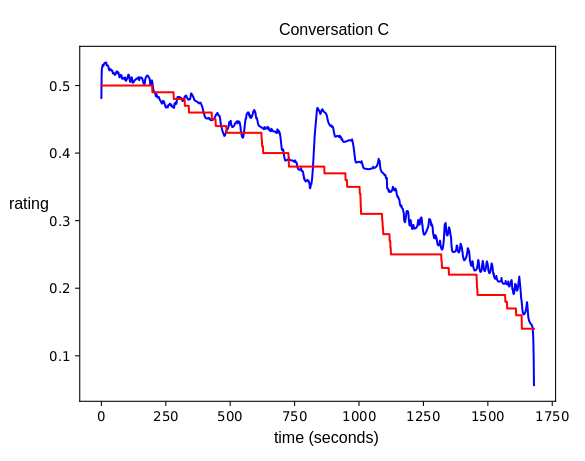
\includegraphics[width=8.4cm]{./Chapitre5/figures/test_ok.png}}
    \end{minipage}
    \begin{minipage}[b]{0.49\linewidth}
        \center
        \centerline{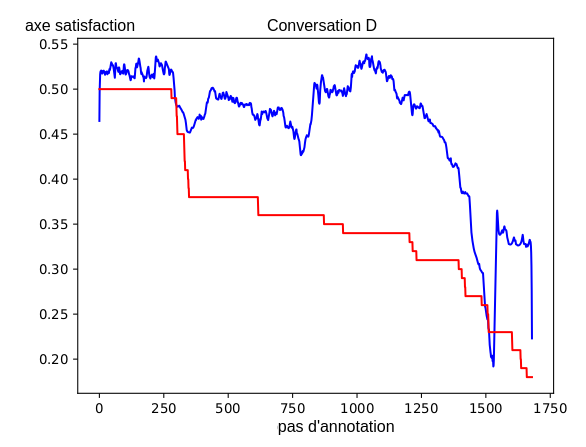
\includegraphics[width=8.4cm]{./Chapitre5/figures/test_not_ok.png}}
    \end{minipage}
    \caption{Prédiction de la satisfaction sur des conversations issues du test. La référence est en rouge, la prédiction en bleu.}
    \label{fig:result7minutes}
\end{figure}


\subsection{Comparaison eGeMAPS et MFCC}
En reconnaissance des émotions, la plupart du temps, la représentation acoustique se concentre principalement sur la capture de la prosodie. C'est pour cette raison que les ensembles de descripteurs dits \textit{experts}, comme par exemple GeMAPS ou IS2009, sont majoritairement utilisés. En effet, comme nous l'avons dit précédemment dans le chapitre~\ref{chapitre3}, ces ensembles de descripteurs sont particulièrement adaptés dans le cadre de la recherche des émotions. En effet, ils permettent une représentation compacte du signal avec un maximum d'informations prosodiques et moins d'informations redondantes que le signal audio.

Cependant, dans notre contexte de capture des conversations, à savoir les conversations téléphoniques, le signal audio peut être plus ou moins dégradé et l'extraction de ces ensembles de descripteurs \textit{experts} peut contenir beaucoup d'erreurs. Par exemple la détection des formants sont généralement peu robuste au bruit, ce qui pénalise le descripteur F0 notamment.%Les extracteurs ne sont, en général, pas prévus pour fonctionner avec des signaux dits dégradés.

Il peut donc être intéressant de comparer l'ensemble eGeMAPS à des descripteurs plus robustes aux signaux dégradés. Nous avons fait le choix de les comparer aux MFCC, décrit au chapitre~\ref{chapitre3}, qui sont plus robustes et leurs extracteurs sont plus fiables dans des contextes de signaux dégradés.

Nous avons décidé de comparer les MFCC issus de deux outils d'extraction différents : OpenSMILE utilisé pour extraire les ensembles IS2009 ou dans notre cas GeMAPS et toutes ses dérivé ainsi que librosa\footnote{https://librosa.github.io/librosa/}. En effet, il est possible d'observer des variations entre plusieurs extracteurs~\cite{Ganchev2005} qui peuvent être liées à la normalisation, au choix de l'échelle Mel, à la fenêtre d'analyse ou encore aux paramètres de FFT. Une fois ces extractions effectuées, nous avons mis en place deux protocoles pour les adapter à nos segments émotionnels de 250~ms :
\begin{itemize}
    \item \textbf{Mfcc-Os} correspond aux MFCC 1 à 13 ainsi qu'à leurs dérivés premières et secondes pour qualifier la dynamique du signal. Ces 39 descripteurs ont été extraits avec l’outil OpenSMILE. Un segment émotionnelest alors représenté par la moyenne et l'écart type de ces 39 descripteurs. Ainsi nous avons un ensemble de 78 descripteurs pour chaque segment émotionnel.
    \item \textbf{Mfcc-lib} correspond aux MFCC 1 à 24 qui sont extraits tous les 10~ms sur des fenêtres de 30~ms. Ces 24 descripteurs ont été extraits avec l'outil librosa. Comme pour les descripteurs précédents, nous avons calculé la moyenne et l'écart type de ces descripteurs au niveau du segment émotionnel. Ainsi nous avons un ensemble de 48 descripteurs pour chaque segment émotionnel. A noter que nons n'avons pas de dérivés dans cet ensemble contrairement à l'ensemble Mfcc-Os.
\end{itemize}

Nous utilisons la meilleure des deux architectures neuronales de la section précédente pour faire notre comparatif, à savoir le biLSTM-4 couches. Les résultats sont regroupés dans le tableau~\ref{tab:egemapsVSmfcc}.

\begin{table}[ht!]
    \centering
    \begin{tabular}{| l | l | l |}
    \hline
    \textbf{Features} &\multicolumn{2}{l|}{\textbf{AlloSat}} \\
    %\hline
    &DEV &TEST \\
    \hline
    eGeMAPS-88  &0.666  &0.431\\
    %eGeMAPS-89  &.619  &\textbf{.542}\\
    eGeMAPS-46  &0.607  &0.354\\
    %eGeMAPS-47  &.574  &.422\\
    Mfcc-lib 48    &\textbf{0.675}  &\textbf{0.510}\\
    Mfcc-Os 78    &0.382  &0.299\\
    \hline
\end{tabular}
    \caption{Comparaison de performance entre descripteurs experts et MFCC. Score CCC rapporté sur les différents ensembles de descripteurs sur le dev et le test d'AlloSat. Le modèle utilisé est le biLSTM-4.}
    \label{tab:egemapsVSmfcc}
\end{table}


Nous pouvons observer tout d'abord une forte différence de score entre les deux types de MFCC. Outre la différence d'implémentation de l'extraction, nous avons mis en place deux protocoles différents pour ces descripteurs (présence ou absence des dérivée, nombre différents de paramètres,...), ce qui peut expliquer cette différence de score. On observe également que les Mfcc-lib ont une meilleure performance que l'ensemble eGeMAPS-89 sur le dev. Ce score semble confirmer que les MFCC sont plus adaptés au signal téléphonique, pour notre corpus, sur la tâche de reconnaissance des émotions.

\subsection{Comparaison CNN et biLSTM}
Dans les travaux menés par Schmitt et al.~\cite{Schmitt2019}, les architectures CNN et biLSTM sont comparées. Le postulat de ces travaux est que nous avons trop tendance à complexifier nos architectures neuronales dans les expériences, et qu'à complexité égale, un système à base de CNN peut faire aussi bien voir mieux qu'un système à base de réseaux récurrents. Le résultat de leur expérimentation confirme cette hypothèse : à complexité égale, leur CNN a de meilleurs performances que leur biLSTM sur le corpus SEWA.

Nous avons donc voulu confronter leur conclusion à notre propre corpus, pour voir si nous pouvions améliorer nos résultats avec des architectures moins complexes que des réseaux récurrents LSTM bidirectionnels. Cela permettrait d'avoir moins de paramètres à apprendre et semble donc pertinent lorsque l'on a des bases de données en quantité limitée, comme avec le corpus AlloSat. En plus des deux architectures biLSTM précédemment expliqué, nous avons mis en place une architecture à base de quatres couches convolutionelles, avec une activation de type ReLU. Comme pour les autres systèmes, un unique neurone en sortie permet de faire la prédiction continue de la valeur de satisfaction. Le CNN est décrit dans la Figure~\ref{fig:CNN}.

\begin{figure}[thb]
  \centering
    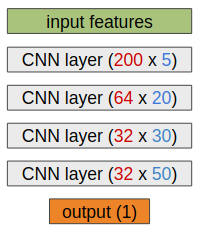
\includegraphics[width=5cm]{./Chapitre5/figures/CNN.png}
    \caption{Schéma de la configuration du système neuronal appelé CNN-4. Le nombre de neurons est en rouge et le filtre recepteur en bleu.}
    \label{fig:CNN}
\end{figure}


Nous avons décidé de comparer nos résultats avec ceux des travaux réalisés sur le corpus SEWA. Pour cela, nous avons utilisé l'ensemble de descripteurs eGeMAPS-47, utilisé par Schmitt et al.~\cite{Schmitt2019}, sur les conversations de taille fixe, donc paddés à 7 minutes. Nous avons donc refait leur expérimentation sur le corpus SEWA et nous l'avons adapté au corpus AlloSat, en partant de l'implémentation de la baseline du challenge AVEC disponible sur github\footnote{https://github.com/AudioVisualEmotionChallenge/AVEC2019}.

Nous avons eu quelques difficultés à faire converger le système convolutif sur nos données. Nous avons fait varier le learning rate, l'initialisation des poids et le nombre d'époque afin de faire converger le système. Certaines initialisation de poids ne permettaient de pas faire converger le système. Nous avons donc fait le choix de présenter dans le tableau~\ref{tab:cnnVSbilstm} la moyenne de cinq modèles dont les poids ont été initialisés différemment (contrôlé par le paramètre \textit{seed}), ainsi que le meilleur des cinq meilleurs modèles sur l'ensemble de développement.

\begin{table}[h]
  \centering
\begin{tabular}{|l|l|l|c|c|c|}
\hline
\multirow{2}{*}{Modèles} & \multirow{2}{*}{Descripteurs} & AlloSat                               & \multicolumn{3}{c|}{SEWA}                                                                                             \\ \cline{3-6}
                         &                               & satisfaction                          & activation                            & valence                               & liking                                \\ \hline
\multicolumn{6}{|c|}{\textbf{Reproduction des résultats avec nos systèmes}}                                                                                                                                              \\ \hline
CNN                      & eGeMAPS-47                    & .178 (.458)                           & \textbf{.528} (.541) & \textbf{.515} (.527) & \textbf{.304} (.321) \\
biLSTM-4                 & eGeMAPS-47                    & \textbf{.437} (.458) & .487 (.527)                           & .428 (.468)                           & .258 (.346)                           \\ \hline
% \multicolumn{6}{|c|}{\textbf{Schmitt et al.~\cite{Schmitt2019} : Train et Dev sur les conversations allemandes}}                                                                                                           \\ \hline
% CNN                      & eGeMAPS-47                    &                                       & .571                                  & .517                                  &                                       \\
% biLSTM-4                 & eGeMAPS-47                    &                                       & .568                                  & .561                                  &                                       \\ \hline
\end{tabular}
\caption{Comparaison des moyennes des scores CCC de cinq systèmes différents sur l'ensemble de développement d'AlloSat et de SEWA.}
 %Nous avons également reporté les résultats issus de Schmitt et al.~\cite{Schmitt2019}}
\label{tab:cnnVSbilstm}
\end{table}


Comme nous pouvons l'observer, nous avons un grand écart entre la moyenne des scores et le score maximal pour le CNN sur le corpus AlloSat. En effet, sur les cinq systèmes, seuls deux ont finis par converger aux alentours de la 80ème époque. Avec un score de $0.437$ de moyenne sur la satisfaction, le système biLSTM-4 donne une meilleure performance sur la moyenne des modèles appris. Cela nous montre que cette architecture est plus stable et moins sujette à la différence de l'initialisation : on a une différence de $0.021$ de score entre le meilleur modèle et la moyenne des scores de cinq modèles différents. Alors que le CNN, même si le meilleur modèle nous donne un score similaire au biLSTM-4, on observe qu'il est bien plus sujet à la différence d'initialisation et donc bien moins stable. De plus, nous n'avons pas réussi à reproduire parfaitement les scores sur le corpus SEWA. Notamment parce que, une fois encore, l'initialisation des réseaux joue un très grand rôle dans le score final.

Pour conclure, nous avons montré que les systèmes à base de couches convolutives ne sont pas tout à fait adaptés à nos données. Ces résultats sont à nuancer notamment à cause de la difficulté de convergence des réseaux convolutifs. Il n'est pas a exclure une mauvaise implémentation de cet apprentissage ou une erreur lors du lancement des expérimentations, malgré tout le soin apporté.

De toute façon, nous voulons à terme travailler sur des séquences de taille non fixe, ce qui ne peut pas être réalisé avec des CNN. Cette volonté correspond aux besoins de l'entreprise qui a besoin d'une analyse de l'émotion sur les conversations entières et non sur une partie uniquement.

Afin de comprendre les différences de scores entre les corpus SEWA et AlloSat, nous avons décider d'enquêter sur les différences inhérentes à ces deux corpus.

\section{Comparaison entre AlloSat et SEWA}
Avant d'étudier les différence intrinsquects aux deux corpus, nous rappelons tout d'abord les scores obtenus par les campagnes AVEC 2018 et 2019 ainsi que ceux obtenus par Schmitt et al., que nous comparons aux scores obtenus sur AlloSat. Le tableau~\ref{tab:allosatVSsewa} présente l'ensemble des résultats comparables que nous avons obtenus sur le corpus AlloSat et le corpus SEWA avec les différents modèles ainsi que les performances obtenues sur SEWA dans l'état de l'art.
%
% Tout d'abord nous avons repris les systèmes décrits dans ces expérimentations pour reproduire les résultats reportés dans les différents articles:
%
% \begin{itemize}
%   \item biLSTM-2 : comme montré dans la figure~\ref{fig:biLSTM}, il s'agit d'un système à deux couches de biLSTM de 64 et 32 neurones. Un seul neurone est utilisé pour la sortie. Ce système est utilisé comme baseline dans les campagnes AVEC~\cite{AVEC2018,AVEC2019} en 2018 et 2019 pour la sous-catégorie \textit{cross-cultural affect}. Il est constitué de 337 473 paramètres.
%   \item biLSTM-4 : comme montré dans la figure~\ref{fig:biLSTM}, il s'agit d'un système à quatre couches de biLSTM de 200, 64, 32 et 32 neurones. Un seul neurone est utilisé pour la sortie. Ce système est utilisé dans les travaux de Schmitt et al.~\cite{Schmitt2019}. Il est constitué de 702 593 paramètres.
% \end{itemize}

\begin{table}[ht!]
      \centering
      \begin{tabular}{| l| l |l |c | c | c |}
          \hline
          \textbf{Modèles} &\textbf{Descripteurs} &\textbf{AlloSat-Dev} &\multicolumn{3}{c |}{\textbf{SEWA-Dev}} \\ \cline{3-6}
          & &satisfaction &activation &valence &liking \\
          \hline
          \multicolumn{6}{| c |}{Nos systèmes : pour SEWA Train et Dev sur les conversations allemandes} \\
          \hline
           \rowcolor{Red}
           CNN       &eGeMAPS-47 &.178 (.458) &\textbf{.528} (.541) &\textbf{.515} (.527) &\textbf{.304} (.321)  \\
            \rowcolor{Red}
           biLSTM-4  &eGeMAPS-47 &.437 (.458) &.487 (.527) &.428 (.468) &.258 (.346)  \\
          \rowcolor{Green}
          biLSTM-2 &eGeMAPS-88  &.480 (.564) &.280 (.357) &.174 (.212) &.095 (.171) \\
          \rowcolor{Green}
          biLSTM-2 &Mfcc-Os     &.364 (.439) &.395 (.438) &.325 (.373) &.158 (.208) \\
           \rowcolor{Blue}
          biLSTM-2 &eGeMAPS-88*  &.480 (.564) &.244 (.273) &.118 (.155) &.082 (.132) \\
          \rowcolor{Blue}
          biLSTM-2 &Mfcc-Os*     &.364 (.439) &.325 (.326) &.186 (.192) &.125 (.126) \\
          biLSTM-4 &eGeMAPS-88  &.564 (.634) &.316 (.429)  &.237 (.309) &.119 (.188) \\
          biLSTM-4 &Mfcc-lib    &\textbf{.666} (.675) &.489 (.501) &.449 (.464) &.124 (133) \\
          biLSTM-4 &Mfcc-Os &.374 (.382) &- &- &- \\
          \hline
          \multicolumn{6}{| c |}{AVEC 2018 : Train et Dev sur les conversations allemandes~\cite{AVEC2018}} \\
          \hline
          \rowcolor{Green}
          biLSTM-2 &eGeMAPS-88 & &(.124)  &(.112) &(.001) \\
          \rowcolor{Green}
          biLSTM-2 &Mfcc-Os    & &(.253)  &(.217) &(.136) \\
           \hline
          \multicolumn{6}{| c |}{AVEC 2019 : Train et Dev sur les conversations allemandes et hongroises~\cite{AVEC2019}} \\
          \hline
          \rowcolor{Blue}
          biLSTM-2 &eGeMAPS-88* & &(.371) &(.286) &(.159) \\
          \rowcolor{Blue}
          biLSTM-2 &Mfcc-Os*    & &(.326) &(.187) &(.144) \\
           \hline
           \multicolumn{6}{| c |}{Schmitt et al. : Train et Dev sur les conversations allemandes~\cite{Schmitt2019}} \\
           \hline
           \rowcolor{Red}
           CNN      &eGeMAPS-47   & &(.571)  &(.517) & \\
           \rowcolor{Red}
           biLSTM-4 &eGeMAPS-47   & &(.568)  &(.561) & \\
           \hline
      \end{tabular}
      \caption{Comparaison des scores moyens de CCC sur les corpus AlloSat et SEWA selon quatre dimensions émotionnelles : la satisfaction, l'activation, la valence et le liking. Nos scores correspondent à la moyenne des scores de 5 systèmes appris avec des initialisations aléatoires différentes et entre parenthèses nous retrouvons le score du meilleur des modèles. Nous reportons également les résultats inclus dans les papiers~\cite{AVEC2018,AVEC2019,Schmitt2019}, qui constituent notre base de comparaison. Ces scores correspondent au meilleur de leur expérimentation, c'est pour cela qu'ils sont notés entre parenthèses, puisqu'à comparer avec les scores des meilleurs modèles notés entre parenthèses dans nos résultats.
      *L'entrainement et les prédictions sont réalisés sur les conversations allemandes et hongroises. Sans le sigle, l'entrainement et les prédictions sont réalisés sur les conversations allemandes uniquement.
      Les couleurs permettent de repérer les différentes expérimentations comparables.}
      \label{tab:allosatVSsewa}
  \end{table}


%Les résultats sont disponibles dans le tableau~\ref{tab:allosatVSsewa}.
 L'initialisation étant un facteur important dans le score final des systèmes, nous avons fait le choix de présenter à la fois la moyenne de cinq systèmes initialisés aléatoirement et le meilleur de ces cinq systèmes (score indiqué entre parenthèses dans le tableau). Comme nous pouvons l'observer, les résultats de nos modèles sont comparables à ceux obtenus dans les différentes baselines sur le corpus SEWA. Ils sont meilleurs que ceux diffusés lors de la campagne de 2018 mais moins performant que ceux de la campagne 2019. Les auteurs de la campagne ont eux-même reconnus que des variations de scores peuvent être observées en fonction de l'initialisation.

On remarque également que nous n'avons pas réussi à bien reproduire les résultats obtenus par Schmitt et al. sur l'activation et la valence. Ceci peut être dû notamment à l'initialisation mais également à la gestion du délai des annotations qui n'est pas pris en compte dans nos expérimentations. Nos systèmes sont plus performants sur la dimension du \textit{liking}, quelque soit les architectures utilisées.

Nous observons également, en comparant les meilleures performances et les performances moyennes, que le système biLSTM-2 entraîné avec les descripteurs Mfcc-Os sur les conversations allemandes et hongroises (en violet) semble être le moins sensible à l'initialisation des poids. De façon général, le plus grand écart type est observé sur la dimension du \textit{liking}.

Les performances obtenues sur l'axe de satisfaction sont comparables à celles obtenues sur les autres dimensions dans le cas de systèmes à base de réseaux récurrents. Les réseaux convolutifs, comme nous l'avons énoncé auparavant, ne semblent pas convenir à notre corpus. La prédiction de l'axe de satisfaction est plus performante avec des réseaux récurrents que des réseaux convolutifs. Il est donc plus prudent d'utiliser des réseaux récurrents lors de tâches de SER, puisqu'ils semblent plus robustes aux changements d'axe émotionnel et aux changements de corpus. De plus, nous avons eu des difficulté à faire converger les systèmes convolutifs selon les différents paramètres et hyper-paramètres du système.

En se concentrant sur la prédiction de l'axe de satisfaction, le modèle appris avec eGeMAPS-88 ($ccc=0.480$) semble être plus performant que celui appris avec Mfcc-Os ($ccc=0.364$) quand on considère l'architecture biLSTM-2. Cependant, en utilisant le système biLSTM-4, les descripteurs eGeMAPS-47 atteignent également de bons résultats ($ccc=0.437$). Pour conclure sur le meilleur nombre de couches, nous effectuons une dernière expérience avec le système biLSTM-4 et eGeMAPS-88 ($ccc=0.564$) qui obtient notre meilleur résultat. Cette architecture semble être la plus convenable pour l'axe de satisfaction.

De cette expérience, nous concluons que le système biLSTM-4 est la meilleure des trois architectures comparées en ce qui concerne la robustesse à la variabilité induite par l'utilisation de différents corpus d'émotions et d'axe émotionnel. Dans la section suivante, nous détaillons les différences entre les deux corpus qui pourraient expliquer la différence de performance entre les systèmes sur ces deux corpus.

\subsection{Analyse des différences entre SEWA et AlloSat}
Nous souhaitons comprendre pourquoi certaines architectures et certains ensembles de descripteurs fonctionnent sur SEWA et non sur AlloSat et inversement. Pour cela, nous cherchons à rendre les corpus plus semblables.

\subsubsection{Variation de l'annotation : pas de l'annotation, taux d'échantillonnage}
Nos premières hypothèses ont porté sur la durée du pas d'annotation et sur la différence de taux d'échantillonnage entre les deux corpus. Nous avons donc décidé de changer les pas d'annotation des deux corpus pour qu'ils soient comparables. Comme nous avons un corpus annoté toutes les 100~ms (SEWA) et l'autre annoté toutes les 250~ms (AlloSat), nous avons choisi de considérer l'annotation toutes les 500~ms. Pour cela, nous avons utilisé une moyenne glissante, afin de rester cohérent avec les annotations d'origines. Nous avons dans le même temps sur-échantillonné les conversations issues d'AlloSat, afin de se ramener à deux corpus échantillonnés selon le même taux soit 44,1kHz. Nous avons choisi de représenter ces échantillons avec l'ensemble eGeMPAS-47 pour pouvoir être comparable à nos précédentes expérimentations.

Nous souhaitions voir des scores dans la même ordre de grandeur pour trouver des justifications à la différence de scores pointés dans la section précédente entre de même architectures et descripteurs entre les deux corpus.

\begin{table}[htp!]
    \centering
    \begin{tabular}{|l|l||l|l|l|}
        \hline
                    &satisfaction &activation &valence &liking \\
        \hline
        CNN         &.046 (.151)   &.368 (.401) &.375 (.424) &.074 (.089)\\
        biLSTM-4    &.503 (.517)   &.457(.476) &.411(.420) &.248(.267) \\
        \hline
    \end{tabular}
    \caption{Comparaison entre les scores obtenus sur l'ensemble de développement d'AlloSat et de SEWA en prenant en entrée des segments émotionnels de 500~ms. Comparaison réalisé sur deux architectures neuronales : CNN et biLSTM-4.}
    \label{tab:pasAnnotation}
\end{table}


Les résultats, présentés sur le tableau~\ref{tab:pasAnnotation} ne permettent de valider aucunes des deux hypothèses. En effet, les résultats sont comparables aux précédents.

\subsubsection{Variation de l'annotation : intensité de la dynamique}
En comparant les deux corpus, nous remarquons que l'axe de satisfaction varie très lentement dans le temps par rapport à l'activation, la valence et au liking. Cela peut être dû au protocole d'annotation (la souris ou le joystick) et au contenu affectif annoté. Nous avons pour cela introduit un indicateur de la quantité de variation QV. QV est défini par la moyenne du nombre de variation dans les conversations et leur intensité. Cette différence de variation peut être observée sur la figure~\ref{fig:variationAnnot} où la dynamique a été quantifiée : nous retrouvons le nombre de variation dans chaque document en ordonnée avec l'ordre de grandeur de ces variations en abscisse. On remarque que les trois axes dimensionnelles de SEWA varient avec bien plus d'intensité que la satisfaction dans AlloSat.%en utilisant la ZCR sur les deltas des dimensions. C
Cette différence de variation pourrait expliquer la différence d'échelle entre les scores obtenus sur le corpus AlloSat et le corpus SEWA.

\begin{figure}[thb]
  \centering
    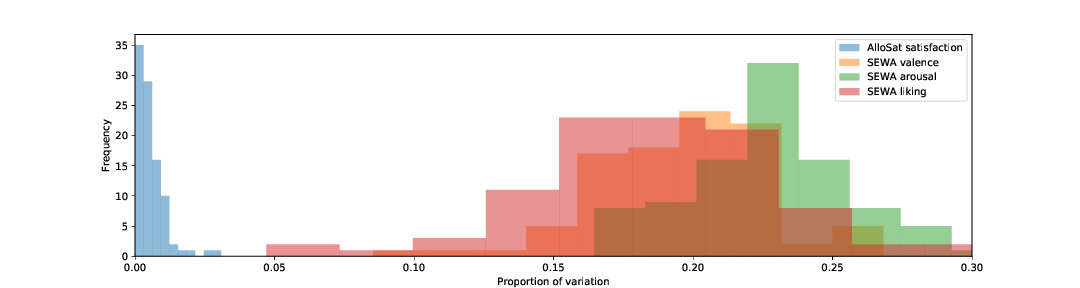
\includegraphics[width=18cm]{./Chapitre5/figures/variation.jpeg}
    \caption{Fréquence des variations dans les annotations des corpus AlloSat et SEWA et leur intensité. La moyenne du nombre de variation de chaque axe dimensionnel est représenté en ordonnée et l'ordre de grandeur de ces variations est donné en abscisse.}
    \label{fig:variationAnnot}
\end{figure}

Pour déterminer si la dynamique dans l'annotation est responsable des mauvais résultats des systèmes convolutifs sur la satisfaction, nous effectuons des expériences supplémentaires avec des références lissées pour l'activation et la valence. Pour mettre en place le lissage, nous avons utilisé une moyenne glissante sur des fenêtres de 200, 500~ms et 1s sur SEWA, ainsi que de 500~ms et 1s sur AlloSat. Les résultats, rapportés dans le tableau~\ref{tab:allosatLisse} montrent qu'aucun de ces procédés ne permettent d'améliorer les performances des systèmes.

\begin{table}[htp!]
    \centering
    \begin{tabular}{| l| l  l  l  | l |}
        \hline
                    &arousal    &valence   &liking &satisfaction \\
        \hline
        original         &.\textbf{528} (.541) &\textbf{.515} (.527) &.304 (.321) &.178 (.458) \\
        200ms           &.512 (.549) &.484 (.492) &\textbf{.340} (.368) &-- \\
        500ms           &.514 (.537) &.491 (.526) &.321 (.379) &.177 (.467) \\
        1000ms          &.519 (.548) &.505 (.518) &.329 (.359) &\textbf{.185} (.475)\\
        \hline
    \end{tabular}
    \caption{Comparaison des scores de développement sur les annotations originales et lissées sur les corpus AlloSat et SEWA. Les descripteurs utilisés sont les eGeMAPS-47 features et le système utilisé est le CNN.}
    \label{tab:allosatLisse}
\end{table}


On peut en conclure que la dynamique faible de l'annotation présente dans le corpus AlloSat n'est pas responsable de la faible performance du système à base de réseaux convolutionels.

\subsubsection{Impact du bruit téléphonique}
Une autre piste que nous avons suivi pour expliquer la dégradation des scores d'AlloSat provient de la modalité téléphonique.
En classification d'images, des études~\cite{Roy2018,Dodge2016} ont montré que l'entraînement de modèles à base de CNN avec des images de mauvaise qualité peut considérablement dégrader les performances des modèles de classification d'images.
Comme AlloSat est composé de conversations téléphoniques, l'enregistrement audio est échantillonné en 8 kHz et il est rempli de bruits : bruit de fond, coupures de son, changement de haut-parleur, etc. Nous émettons donc l'hypothèse qu'AlloSat est trop dégradé pour être bien traité par des réseaux convolutifs.
Pour confirmer notre hypothèse, nous avons sous-échantillonné les données SEWA de 44 kHz à 8 kHz.

Nous proposons également d'ajouter du bruit au jeu de données SEWA, afin de le rendre plus comparable avec le contexte AlloSat. Les bruits d'appels téléphoniques sont principalement composés de bruits de fond tels que les bruits de la rue ou de la circulation.

Pour injecter du bruit dans nos enregistrements, nous avons utilisé la base de données SoundJay~\footnote{https://www.soundjay.com/} et nous avons suivi le processus décrit dans l'article~\cite{Alzqhoul2016}. Trois types de bruits (voiture, rue et conversations de foule) sont ajoutés de manière aléatoire au signal à différents niveaux de volumes (9, 15, 21 décibels). En plus de ces bruits, nous avons fait le choix d'ajouter des voix d'enfants, puisque l'on en entend assez souvent dans le corpus. Les enregistrements résultants ont été vérifiés manuellement pour vérifier si les perturbations auditives sont comparables à celles observées dans AlloSat.

\begin{table}[htp!]
   \centering
   \begin{tabular}{|l| l  l  l|}
       \hline
                   &activation    &valence   &liking \\
       \hline
       %44kHz           &.322 (.415)  &.337 (.440) &.106 (.209) \\
       %8kHz            &.486 (.539) &.495 (.532) &.187 (.289) \\
       %8kHz + noise    &.471 (.497) &.464 (.486) &.204 (.250) \\
       44kHz           &\textbf{.528}  &\textbf{.515} &\textbf{.304} \\
       8kHz            &.486 &.495 &.187 \\
       8kHz + bruit    &.471 &.464 &.204 \\
       \hline
   \end{tabular}
   \caption{Comparaison des scores de développement entre les versions originales du corpus SEWA et les versions dégradées. Les dégradations sont le sous-echantillonage des enregistrement audio et l'ajout de différents bruits. Nous utilisons les descripteurs eGeMAPS-47 ainsi qu'un modèle CNN. L'entrainement et les prédictions sont effectuées sur les conversations allemandes.}
   \label{tab:downsample}
\end{table}


Les résultats, présentés dans le tableau~\ref{tab:downsample}, montrent qu'en dégradant les signaux SEWA (en sous-échantillonnant à 8 kHz et en ajoutant du bruit), nous diminuons les performances. Mais nous sommes loin d'atteindre les mauvaises performances des réseaux convolutifs sur AlloSat.

Toutes nos hypothèses ne nous permettent pas de justifier la différence de score entre AlloSat et SEWA lorsque l'on utilise des réseaux convolutifs. Les bonnes performances obtenues sur SEWA avec le CNN dans nos expérimentations nous font douter que le problème vienne de l'implémentation en elle-même. Le changement de la dimension annotée, les conditions d'enregistrement, le contenu sémantique, la langue, le choix des hyper-paramètres ou encore le protocole mis en oeuvre sont d'autant d'explications possible quant à la différence de performance de ces réseaux sur les deux corpus.

\section{Analyses annexes}
%Comme les résultats que nous avons présenté auparavant nous semblait pertinent, nous avons décidé de faire de plus amples expérimentations sur la totalité des conversations en utilisant les différentes configurations expliquées plus tôt. Nous ne pouvons pas faire d'expérimentations à partir de systèmes à base de CNN, dû à la nature de ce réseau, qui permet de faire des reconnaissances à partir de séquences de taille fixe.

%Nous avons également choisi de changer d'implémentation en passant de l'utilisation de Keras à celle de Pytorch~\cite{pytorch}. En effet cet outil permet de gérer plus en profondeur les paramètres des réseaux et a un temps d'apprentissage fortement diminué.

\subsection{Décalage des annotations dans le temps}

Comme nous l'avons dit précédemment, il est tout à fait possible que les annotations soient décalées dans le temps. En effet, les annotateurs peuvent prendre plus ou moins de temps à annoter la variation d'une émotion.
La question est assez complexe, puisque l'on ne connait pas la distribution des décalages. Ils peuvent être très forts (décalage long) chez un annotateur ou dans une conversation en particulier, et très faible (décalage court) dans d'autres cas. Généralement, on estime que le processus de décision de l'humain prend entre 2 et 4 secondes~\cite{Huang2015,Mariooryad2014}.

Ce décalage a été étudié notamment dans l'article de Schmitt et al.~\cite{Schmitt2019} où des décalages jusqu'à 5 secondes ont été expérimentés, et nous voulons analyser ce phénomène sur les données d'AlloSat.

Nous avons donc mis en place deux décalages : de 2s (soit 8 pas d'annotations) et de 4s (soit 16 pas d'annotations). Ce décalage à \textit{droite} consiste à décaler les annotations des segments émotionnels de $X$ pas d'annotations avec $X=8$ ou $X=16$. Les débuts de conversations, ainsi privés d'annotations, ont été remplacé par une annotation neutre de $0.50$. Les annotations \textit{trop à droite} ont été supprimées des données.

\begin{table}[h]
  \centering
\begin{tabular}{|l|l|l|l|l|l|l|}
\hline
Descripteurs & \multicolumn{2}{l|}{Sans décalage} & \multicolumn{2}{l|}{\begin{tabular}[c]{@{}l@{}}Décalage \\ 2 secondes\end{tabular}} & \multicolumn{2}{l|}{\begin{tabular}[c]{@{}l@{}}Décalage \\ 4 secondes\end{tabular}} \\ \hline
              & DEV             & TEST             & DEV                     & TEST           & DEV                     & TEST           \\ \hline
eGeMAPS\_88  & \textbf{0.666}   & \textbf{0.431}  & 0.603               & 0.293              & 0.489               & 0.230               \\ \hline
eGeMAPS\_89  & \textbf{0.619}   & \textbf{0.542}  & 0.601               & 0.303              & 0.502               & 0.278              \\ \hline
f\_eGeMAPS\_46  & \textbf{0.607}   & \textbf{0.354}  & 0.523               & 0.346              & 0.557               & 0.324              \\ \hline
f\_eGeMAPS\_47  & \textbf{0.574}   & \textbf{0.422}  & 0.477               & 0.245              & 0.450                & 0.231              \\ \hline
\end{tabular}
\caption{Score CCC des systèmes de reconnaissance des émotions d'une architecture neuronale bilstm à quatre couches en fonction du décalage des annotations.}
\label{tab:decalage}
\end{table}


Le tableau~\ref{tab:decalage} nous donne les résultats des systèmes utilisant l'architecture neuronale du biLSTM-4, présenté précédemment. Nous pouvons observer que quelque soit l'ensemble de descripteur utilisé, les scores sur les données de dev et de test sont toujours meilleurs sans décalage. Même si le décalage permet d'atteindre des scores sur l'ensemble de développement avoisinant ceux sans décalage, on remarque que le pouvoir de généralisation du modèle en pâtit grandement. Nous avons également essayer de plus forts décalages, à savoir 8 et 12 secondes, mais les résultats ne font que se dégrader. Ces observations sont en adéquation avec celles des travaux de Schmitt et al. L'inconsistance dans le décalage humain ou un décalage inférieur peuvent être des hypothèses valable pour expliquer cette dégradation.

Pour notre corpus et en utilisant des architectures de type biLSTM, le décalage des annotations ne permet pas d'améliorer les scores de reconnaissance des émotions.

\subsection{Fonction de coût}
Comme nous l'avons vu précédemment dans le chapitre~\ref{chapitre3}, le CCC est un outil d'évaluation très utilisé dans la reconnaissance d'émotions continues. Les challenges AVEC~\cite{AVEC2018} ont notamment contribué à la standardisation de l'utilisation de cette métrique pour évaluer les systèmes de reconnaissance continue d'émotion. Pour rappel, le CCC se calcule selon l'équation~\ref{eq:CCCscore}.

\begin{equation}
   \rho = \frac{2\rho\sigma_x\sigma_y}{\sigma_x^2 + \sigma_y^2 + (\mu_x - \mu_y)^2}
\label{eq:CCCscore}
\end{equation}

Si on regarde l'équation, quand la référence est constante sur la totalité de la conversation, $\sigma_y = 0$ et donc le coefficient est égal à zéro. De façon plus générale, quand la référence varie peu, le CCC va s'approcher de zéro, même si la prédiction est quasiment parfaitement synchronisée à la référence.

On peut donc en conclure que la fonction de coût va pénaliser les conversations où la référence varie peu ($\sigma_y \simeq 0$) et que le système ainsi entraîné aura du mal à prédire correctement de telles références.

\begin{table}[htp]
\centering
\begin{tabular}{| l | l l |}
    \hline
    \textbf{Descripteurs} &\multicolumn{2}{c|}{\textbf{AlloSat}} \\
      &\textit{l-ccc}   &\textit{l-rmse}  \\
    \hline
    eGeMAPS-47  &.437 &.381       \\
    eGeMAPS-88  &.564 &.514       \\
    Mfcc-lib    &.675  &\textbf{.698} \\
    Mfcc-Os     &.382   &405      \\
    \hline
\end{tabular}
\caption{Score CCC des systèmes de reconnaissance des émotions sur l'ensemble de développement d'AlloSat. On compare l'utilisation de deux fonctions de coût \textit{l-ccc} et \textit{l-rmse}. Les systèmes sont issus de l'architecture neuronale biLSTM-4.}
\label{tab:cccVSrmse}
\end{table}


Nous avons comparé les scores obtenus en utilisant la RMSE comme fonction de coût que nous avons introduit au chapitre~\ref{chapitre3} pour palier à ce problème. Le tableau~\ref{tab:cccVSrmse} résume les différences de scores calculés sur le dev.

Comme nous pouvons l'observer, les scores sont globalement meilleurs si on utilise la fonction de coût l-ccc. On remarque cependant que dans le cas des descripteurs \textit{Mfcc-lib}, l'utilisation de la fonction de coût l-rsme permet d'améliorer les résultats. Cependant lorsque l'on regarde la prédiction effective sur les conversations, on se rend compte que les prédictions ne sont pas homogènes en terme de qualité, comme en témoigne la Figure~\ref{fig:cccVSrmse} où à gauche nous retrouvons une prédiction peu satisfaisante avec un score CCC de $0.564$ alors qu'à droite nous retrouvons une très bonne prédiction avec un score CCC de $0.903$.

\begin{figure}[h]
        \centering
        \begin{subfigure}{.49\textwidth}
          \centering
          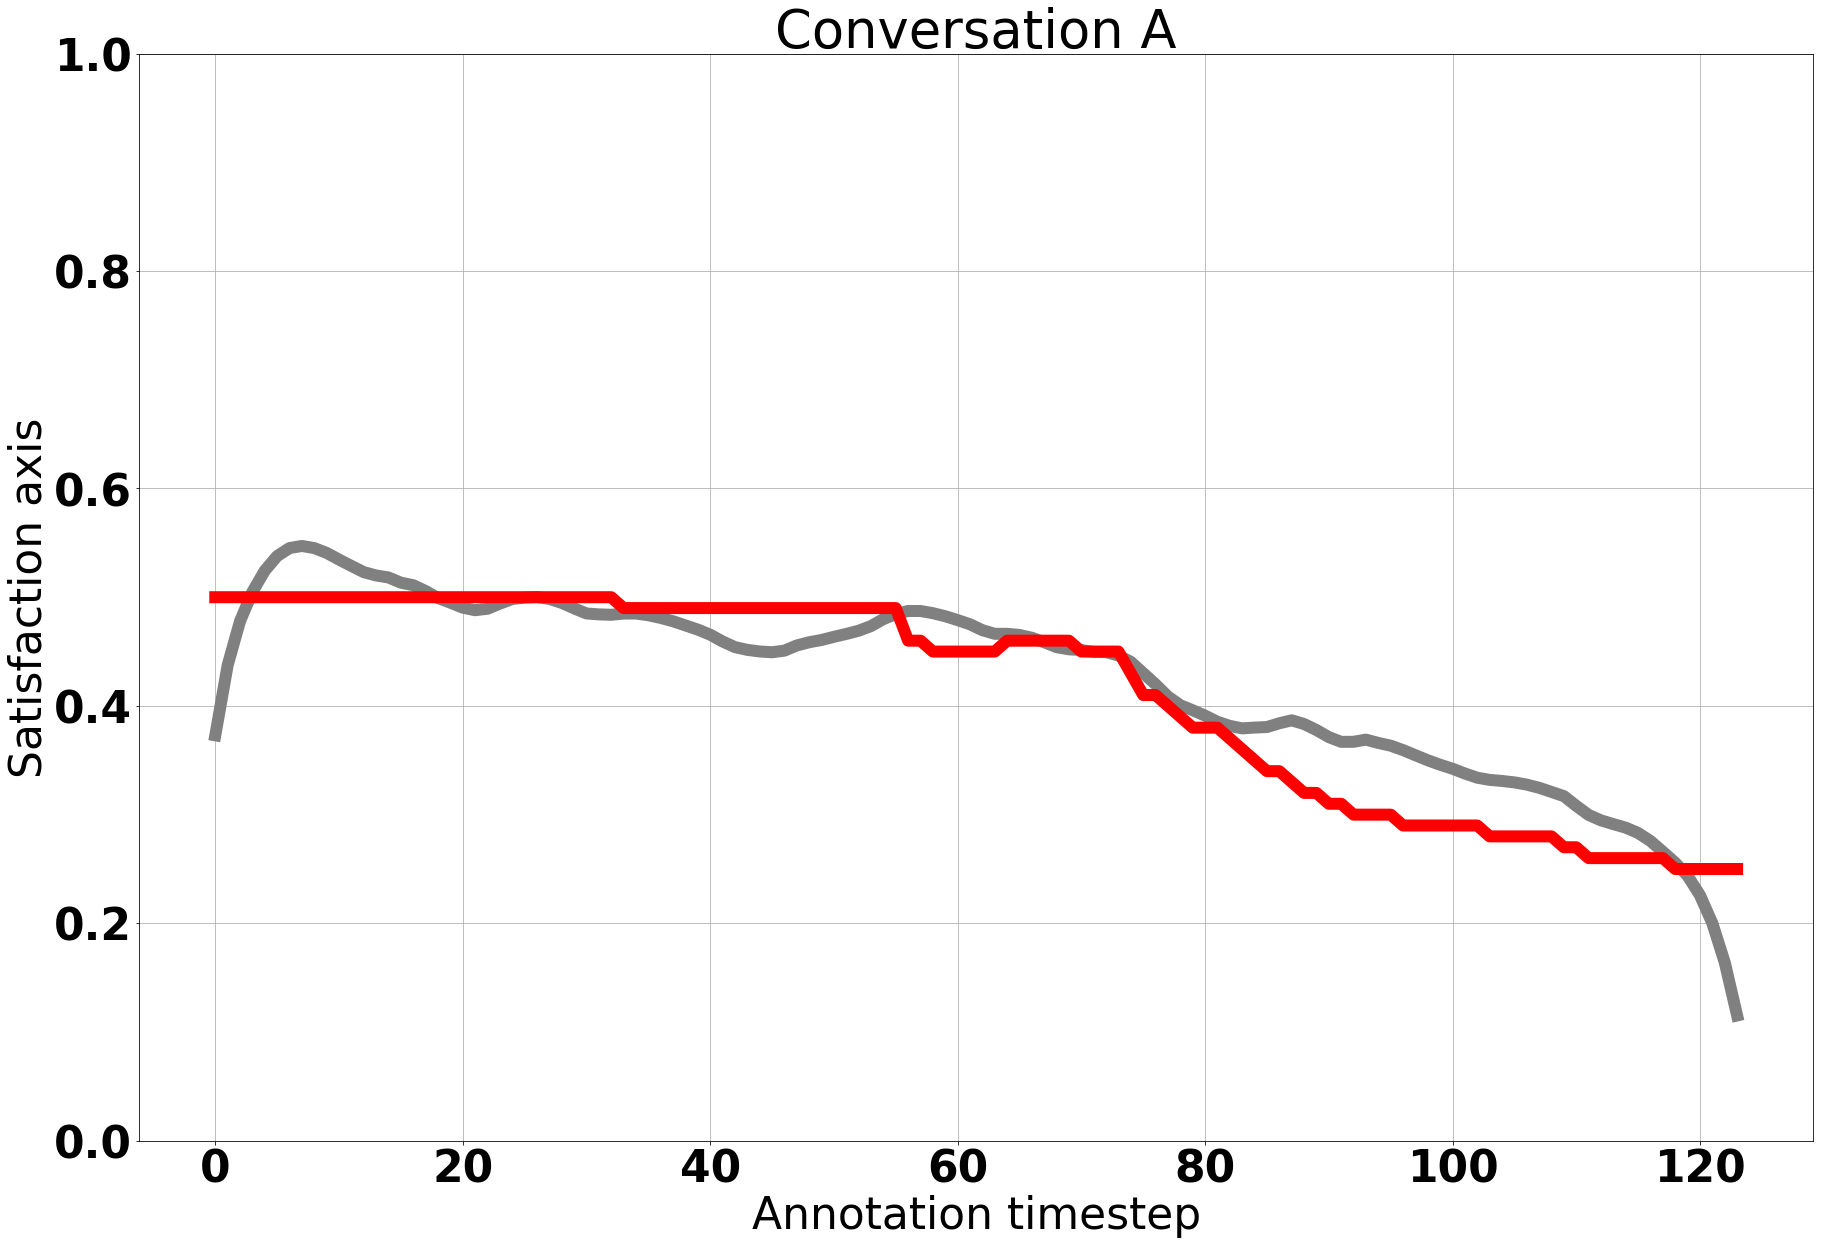
\includegraphics[width=.99\linewidth]{./Chapitre5/figures/cccVSrmse1.png}
        \end{subfigure}
        \begin{subfigure}{.49\textwidth}
          \centering
          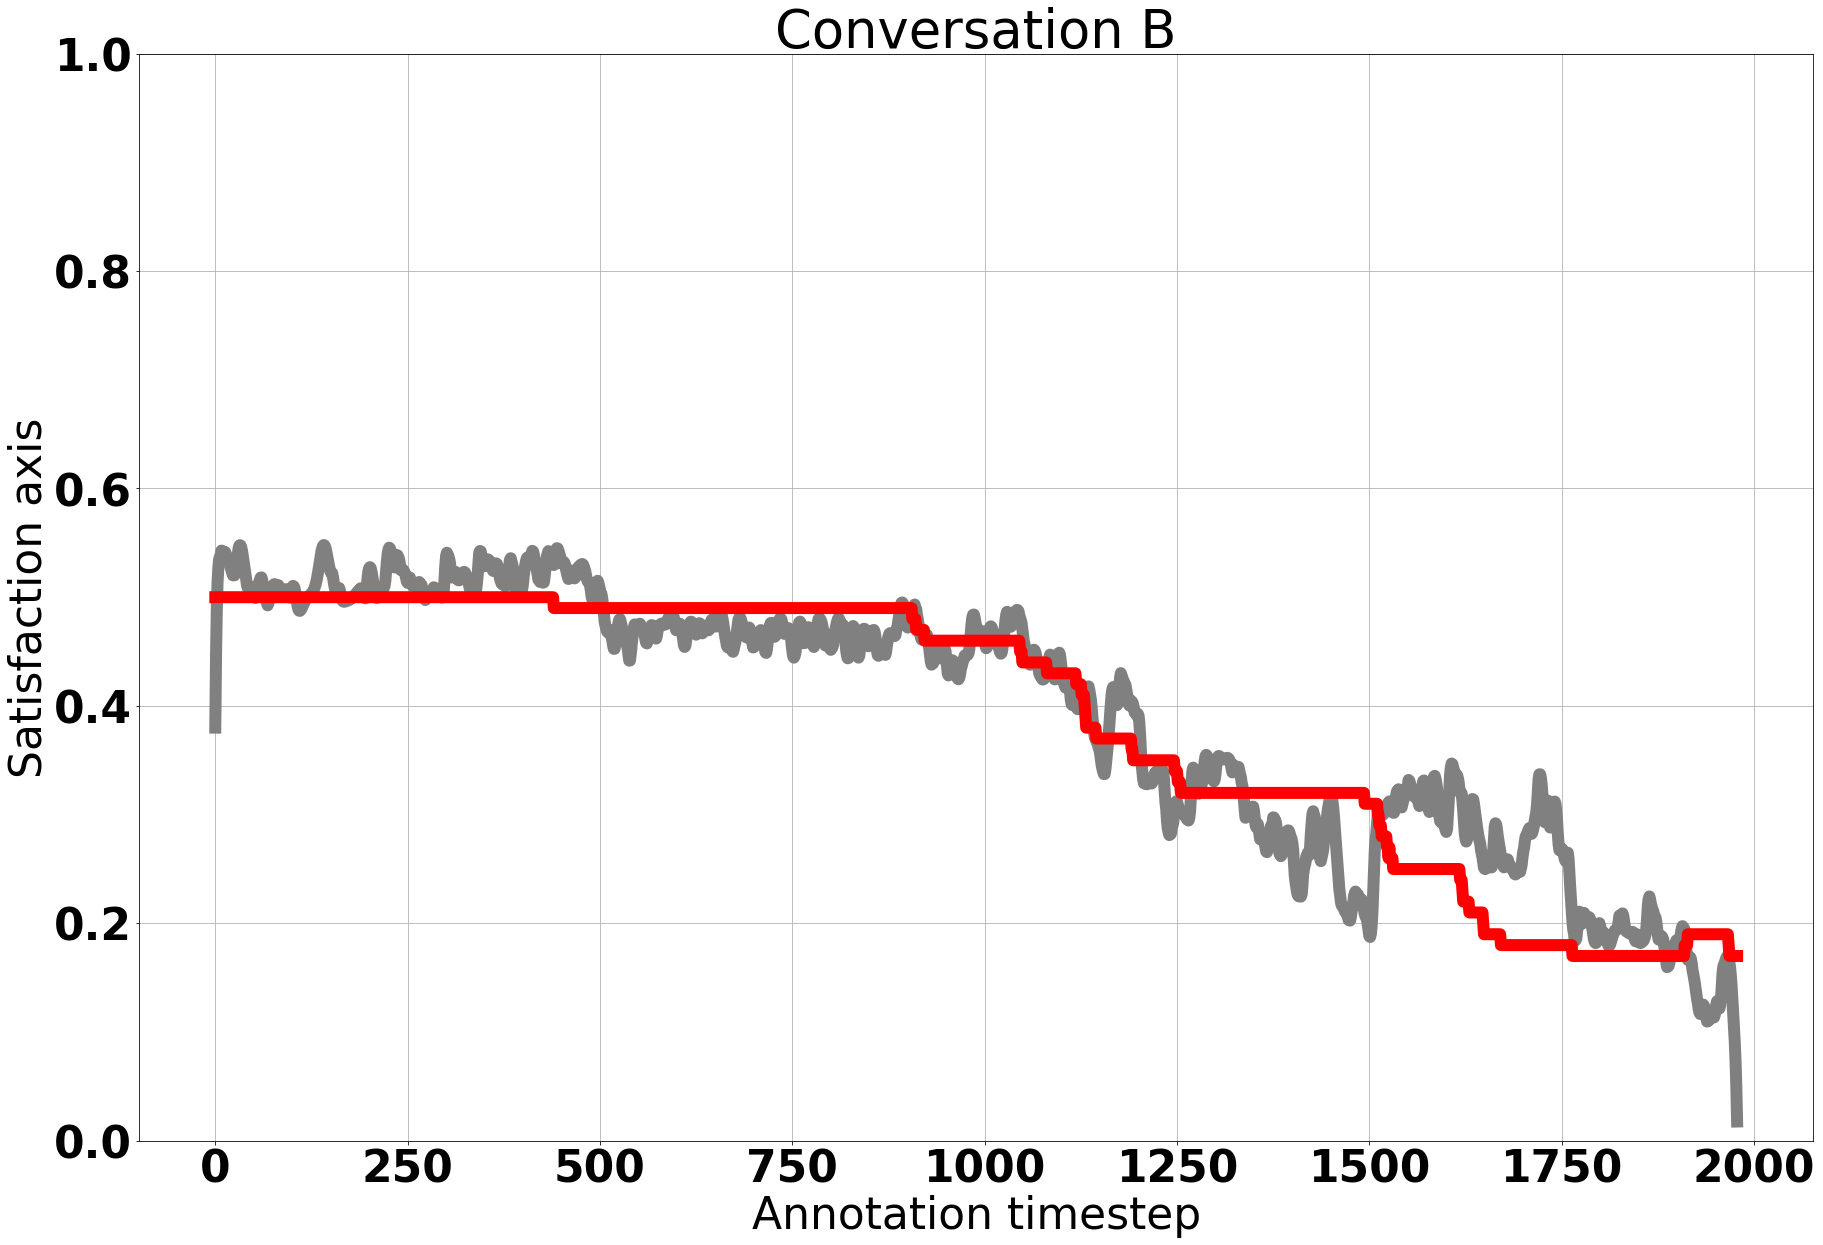
\includegraphics[width=.99\linewidth]{./Chapitre5/figures/cccVSrmse2.png}
        \end{subfigure}
        \caption{Evolution des prédictions (grises) et des références (rouge) de deux conversations provenant de l'ensemble de test d'AlloSat. $ccc(A) = 0.564$, $ccc(B) = 0.903$.}
        \label{fig:cccVSrmse}
    \end{figure}


Nous avons donc décidé de mettre en place un post-traitement afin de lisser les courbes de prédiction, pour avoir une meilleure représentation des émotions.

\subsection{Post-traitement : lissage des prédictions}
Nous avons décidé de mettre en place un lissage des prédictions. Pour cela, nous avons utilisé l'algorithme de lissage Savistky-Golay~\cite{Savitzky1964} avec un degré polynomial de zéro. Bien qu'ancien, cet algorithme est toujours autant utilisé dans le traitement des signaux. C'est une extension de la moyenne glissante, qui est utilisée pour atténuer les pics des signaux en approximant un polynôme pour chaque fenêtre de la moyenne glissante, ici un polynôme de degré zéro. Nous avons fait le choix de ce degré puisque c'est celui qui va lisser au maximum la courbe.
%It has been applied to the series of data with a window of 101, again, to try flatten the curve as much as possible.

Nous avons donc appliqué ce lissage sur les prédiction du meilleur système obtenu jusque là, les résultats sont disponibles dans le tableau~\ref{tab:lissage}.


\begin{table}[h]
    \centering
        \begin{tabular}{| l | l l | l l |}
        \hline
        \textbf{Descripteurs} &\multicolumn{2}{c|}{\textbf{Dev}}& \multicolumn{2}{c |}{\textbf{Test}}\\
        &Non lissé &Lissé &Non lissé &Lissé \\
        \hline
        Mfcc-lib (\textit{l-rmse})    &.698 &\textbf{.719} &.513 &\textbf{.570}  \\
        \hline
    \end{tabular}
    \caption{Scores CCC avec et sans lissage calculés sur les ensembles de développement et de test d'AlloSat. Score issu du meilleur modèle : système biLSTM-4, descripteurs Mfcc-lib et fonction de coût RMSE.}
    \label{tab:lissage}
\end{table}


Nous pouvons observer qu'il s'agit du meilleur score jamais obtenu sur les prédictions de l'axe de satisfaction. De même, la figure~\ref{fig:cccVSrmse} permet de se rendre compte du profit que nous tirons du lissage. On l'observe sur la figure de droite, tracée en bleu.

Grâce à ce lissage, nous obtenons de très bons scores : $0.719$ pour l'ensemble de développement et $0.570$ pour le test. Nous utilisons ses scores comme référence sur le corpus AlloSat dans la suite de nos travaux.%Nous avons voulu confronter ces scores à ceux obtenus dans l'état de l'art, sur le corpus SEWA.


\section{Conclusion}
Dans ce chapitre, nous avons décrit les différents choix que nous avons considéré pour construire un modèle de reconnaissance des émotions. Nous avons d'abord présenté la reconnaissance d'émotions discrètes puis continues. Nous avons également validé nos expérimentations et la pertinence de notre corpus en le comparant au corpus de l'état de l'art SEWA.

Nous pouvons conclure que le meilleur système de reconnaissance des émotions continues utilise un réseau de neurones récurrents, un ensemble de descripteur tiré des MFCC, sur lequel nous appliquons un post-traitement de lissage.

Cependant comme nous l'avons dit précédemment, la modalité acoustique n'est pas la seule permettant de retrouver les états émotionnels. Dans le prochain chapitre, nous allons mesurer l'apport de la modalité linguistique ainsi que l'apport de descripteurs pré-entrainés de type BERT.
